\documentclass[dvipdfmx,autodetect-engine,12pt]{jsarticle}
\usepackage[utf8]{inputenc}

\usepackage{amsmath,amsfonts,amssymb}
\usepackage{graphicx}
\usepackage[dvipdfmx]{hyperref}
\usepackage{pxjahyper}%these two come together
\usepackage[dvipdfmx]{color}
\usepackage{braket}%dirac notation
\usepackage{wrapfig}
\usepackage{here}
\usepackage{tabularx, dcolumn}
\usepackage{subfigure}
\usepackage{cases}
\usepackage{bigints}%インテグラルで大きくする
\usepackage{mathtools} 
\hypersetup{hidelinks}
\interfootnotelinepenalty=10000 % this is to keep a footnote in a single page
\usepackage{bm}%ベクトル記号
\usepackage{ascmac} %囲い
%%%%%%
\usepackage{tikz}
\usepackage{amsmath}
\usepackage{cases}%連立方程式


%%%%%%newcomand
\newcommand{\be}{\begin{equation}}
\newcommand{\ee}{\end{equation}}
\newcommand{\nn}{\notag \\}

\usepackage{mdframed}%ページをまたぐ    
\newmdenv[skipabove=6mm, skipbelow=4mm]{kotak}


\newtheorem{definition}{定義}[section]
\newtheorem{theorem}[definition]{定理}
\newtheorem{proof}{証明}
\newtheorem{request}[definition]{要請}
\newtheorem{prop}[definition]{命題}
\newtheorem{these}[definition]{仮定}
\newtheorem{lemma}[definition]{補題}
\newtheorem{postlate}[definition]{公理}

%sectionの大きさを変更する
%\usepackage[explicit]{titlesec}

%operator
\newcommand{\hH}{{\hat{H}}}%ハミルトニアン
\newcommand{\hHt}{{\hat{\mathcal{H}}}}%ハミルトニアン
\newcommand{\hU}{{\hat{U}}}
\newcommand{\hM}{{\hat{M}}}
\newcommand{\hN}{{\hat{N}}}
\newcommand{\hA}{{\hat{A}}}
\newcommand{\hB}{{\hat{B}}}
\newcommand{\hO}{{\hat{O}}}
\newcommand{\hAd}{{\hat{A}^\dag}}
\newcommand{\ha}{{\hat{a}}}
\newcommand{\hb}{{\hat{b}}}
\newcommand{\had}{{\hat{a}^\dag}}
\newcommand{\hpsi}{{\hat{\psi}}}
\newcommand{\hpsid}{{\hat{\psi}^\dag}}
\newcommand{\hrho}{{\hat{\rho}}}
\newcommand{\hsig}{{\hat{\sigma}}}
\newcommand{\hx}{{\hat{x}}}
\newcommand{\hy}{{\hat{y}}}
\newcommand{\hz}{{\hat{z}}}
\newcommand{\hX}{{\hat{X}}}
\newcommand{\hY}{{\hat{Y}}}
\newcommand{\hZ}{{\hat{Z}}}
\newcommand{\hp}{{\hat{p}}}
\newcommand{\hvp}{{\hat{\bm p}}}

%%%%%%%%%%%%%%%%%%%%%%%%%%%%%%%%%%%%%%
%%%%%%%%%%%%%%%%%%%%%%%%%%%%%%%%
% USER SPECIFIED COMMANDS
%%%%%%%%%%%%%%%%%%%%%%%%%%%%%%%%
\newcommand{\ie}{i.e.}
\newcommand{\eg}{e.g.}
\newcommand{\etal}{\textit{et al.}}
\newcommand{\e}{\textrm{e}} % Exponential
\newcommand{\hc}{\text{h.c.}} % Hermitian conjugate

\newcommand{\nbar}{\bar{n}}
\newcommand{\adag}{\hat{a}^\dagger}
\newcommand{\adagsq}{\hat{a}^{\dagger 2}}
\newcommand{\hata}{\hat{a}}

\newcommand{\jg}[1]{{\color{orange}#1}}
\newcommand{\dr}[1]{{\color{red}#1}}
\newcommand{\rg}[1]{{\color{MidnightBlue}#1}}
\newcommand{\filler}[1][1]{{\color{gray}\lipsum[1-#1]}}
%%%%%%%%%%%%%%%%%%%%%%%%%%%%%%%%%%%%%

%\vector
\newcommand{\vr}{{\bm{r}}} %vector r
\newcommand{\vP}{{\bm{P}}} %vector r
\newcommand{\vphi}{{\varphi(t,\bm{r})}}

%

\newcommand{\tr}{\mathrm{Tr}}
\newcommand{\diag}{\mathrm{diag}}
\newcommand{\rint}{\mathrm{int}}
\newcommand{\tot}{\mathrm{tot}}


\newcommand{\YM}[1]{\textcolor[rgb]{1, 0.1, 0.1}{#1}}
\newcommand{\YMdel}[1]{\sout{#1}}
%\newcommand{\YMdel}[1]{\textcolor[rgb]{1, 0.1, 0.1}{\sout{\textcolor{black}{#1}}}}
\newcommand{\KM}[1]{\textcolor[rgb]{0.1, 0.1, 1}{#1}}
\newcommand{\KMdel}[1]{\textcolor[rgb]{0.1, 0.1, 0.9}{\sout{\textcolor{black}{#1}}}}


\makeatletter
\title{統計力学}



\begin{document}
\maketitle


\tableofcontents
%目の保護用
%\pagecolor{black}
%\color{white}
%%%%%%%%%%%%%%%%%%%%%

\part{ミクロカノニカルアンサンブル}
\section{平衡状態の本質}
\subsection{等重率の原理}
平衡状態のマクロな性質とは「典型的な状態」が共通にもっている性質のことである.我々が共通の性質を知りたいのならば,方針として,「例外的状態を含めて,取りうる状態すべてについて平均をとる」ことである.この方針は例外的な状態を含めても,圧倒的大多数が典型的な状態であるから,平均的な性質に与える影響は無視できるはずである.つまり,等確率になるモデルを考えれば,平均を考えることができる.そこで,次に示す等重率の原理\footnote{%
原理と名前についているが,本当に成立しているかどうかは証明できない.
}
あるいは等確率の原理と呼ばれる確率モデルを考える.
 \begin{itembox}[l]{等確率の原理}
「エネルギーが$E$となる各力学的な状態は,等確率で出現する.」
\end{itembox}
これは,「共通の性質」を抽出するための理論的方策である.
\section{小正準集合の方法}
\subsection{ミクロカノニカルアンサンブル}
 \begin{itembox}[l]{小正準集合(ミクロカノニカルアンサンブル)}
$E$に$[E,E+\delta E]$と幅を持たせる.小正準集合とは「$N$,$V$,$E\sim E+\delta E$を指定したときに,各々の取りうる力学的状態が等確率(定数)で出現する確率モデル」である.
\end{itembox}
上の文章をそのまま式で表そう.状態$(N,V,[E+\delta E])$を指定したときにある力学的な状態「$r$」が出現する確率を$p_{N,V,E}(r)$とすると
\begin{equation}
p_{(N,V,E)}(r)=A\mbox{(定数)}
\end{equation}
とかける.すべての力学状態に対する足し上げを行うと
  \begin{eqnarray*}
\begin{split}
\displaystyle\sum_{r}p_{(N,V,E)}(r)=\displaystyle\sum_{r}A=A\displaystyle\sum_{r}1
  \end{split}
\end{eqnarray*}
$\displaystyle\sum_{r}1$は全状態数になっているから,$(N,V,[E+\delta E])$をとる状態数を$W(N,V,E)$とおくと,
  \begin{eqnarray*}
\begin{split}
\displaystyle\sum_{r}p_{(N,V,E)}(r)=A\displaystyle\sum_{r}1=A\ W(N,V,E)
  \end{split}
\end{eqnarray*}
となる.これが1と等しいから,
  \begin{eqnarray*}
\begin{split}
A=\frac{1}{W(N,V,E)}
  \end{split}
\end{eqnarray*}
となり,
\begin{equation}
\label{p1}
p_{(N,V,E)}(r)=
{}
\begin{cases}
\dfrac{1}{W(N,V,E)}\\[20pt]
0
    \end{cases}
\end{equation}
を得る.


























%
\subsection{微視的状態数と分布関数}
\begin{align}
\fbox{
a=u
%\begin{tabular}{l}
%\end{tabular}
}
\end{align}
位相空間のなかの
\begin{align}
d^N\Gamma=d\bm{q}^Nd\bm{p}^N=dq_1\cdots dq_{3N}dp_1\cdots dp_{3N}
\end{align}
なる体積をもつ微小領域の中には,
\begin{align}
\frac{d^N\Gamma}{(2\pi\hbar)^{3N}}
\end{align}
だけの個数の,準古典的な状態が含まれることになる.
まず,位相空間上でHamiltonianによって定まるエネルギーが$0$から$E$までの間に,一様に微視的状態数が存在しているとし,
その間に含まれる微視的状態の総数を求める.それを$W_0(E)$とすれば,
\begin{align}
\label{mc1}
\fbox{
$W_0(E)=\dfrac{1}{(2\pi\hbar)^{3N}}\displaystyle\int_{0\leq H_N\leq E}d^N\Gamma\Theta\bigl(E-H_N(\bm{q},\bm{p})\bigr)$
}
\end{align}
で与えられる.ただし,右辺の積分は
\begin{align}
\int\cdots\int_{0\leq H_N\leq E}\frac{dq_1dp_1}{(2\pi\hbar)}\cdots\frac{dq_{3N}dp_{3N}}{(2\pi\hbar)}
\end{align}
の略記である.ここで,$\Theta\bigl(E-H_N(\bm{q},\bm{p})\bigr)$はHeavisideの階段関数
 \begin{equation}\label{heav}
\Theta\bigl(E-H_N(\bm{q},\bm{p})\bigr)
  = \begin{cases}
      1  & (E\geq H_N(\bm{q},\bm{p}))\\[15pt]
      0 & (E<H_N(\bm{q},\bm{p}))
    \end{cases}
\end{equation}
である.(\ref{heav})はエネルギーが$E$以上となるような$H_N(\bm{q},\bm{p})$ではその値が0となるから,(\ref{heav})をつかって,状態数$W_0(E)$を記述することができる.また,エネルギーが$E$以下の状態数を求めたい場合に(\ref{mc1})の表記は便利である.\\
%
 エネルギー$E$は巨視的な量で連続値であるから,$W_0(E)$は変数$E$で微分することができる.$W_0(E)$を$E$で微分すると,$E$という点での微視的状態の密度$w(E)$は
\begin{align}
\label{mc2}
w(E)=\frac{\partial W_0(E)}{\partial E}
&=
\dfrac{1}{(2\pi\hbar)^{3N}}\int_{0\leq H_N\leq E}d^N\Gamma
\frac{\partial\Theta\bigl(E-H_N(\bm{q},\bm{p})\bigr)}{\partial E}\notag\\[10pt]
&=
\dfrac{1}{(2\pi\hbar)^{3N}}\int_{0\leq H_N\leq E}d^N\Gamma
\delta\bigl(E-H_N(\bm{q},\bm{p})\bigr)
\end{align}
となる.ここで,公式$\dfrac{\partial \Theta(x)}{\partial x}=\delta(x)$を用いた.状態密度$w(E)$は単位エネルギーあたりの状態数という意味をもつ.\\
 エネルギー$E$と$E+\delta E$の間にあるすべての可能な微視的状態の数は,エネルギーがそれぞれ$E+\delta E$,$E$以下の,微視的状態の総数$W_0(E+\delta E)$と$W_0(E)$の差を用いて,
\begin{align}
\label{mc3}
W(E,\delta E)=W_0(E+\delta E)-W_0(E).
\end{align}
(\ref{mc3})の右辺を$E$の周りでTaylar展開し1次までとれば,
\begin{align}
W(E,\delta E)=\frac{\partial W_0(E)}{\partial E}\delta E
\end{align}
となる.状態密度$w(E)$を用いれば,エネルギー$E$と$E+\delta E$の間にあるすべての可能な微視的状態の数は
\begin{align}
\label{mc4}
\fbox{
$W(E,\delta E)=w(E)\delta E$
}
\end{align}
となる.一方,${}^N\Gamma$空間上での微視的状態数と位相体積の関係は
\begin{align}
\label{mc5}
\fbox{
$W(E,V,N,\delta E)=\dfrac{1}{(2\pi\hbar)^{3N}}\displaystyle\int_{E\leq H_N\leq E+\delta E}d^N\Gamma
=\dfrac{1}{(2\pi\hbar)^{3N}}\displaystyle\int_{E\leq H_N\leq E+\delta E}d^N\Gamma\Omega({}^N\Gamma)$
}
\end{align}
で与えられる.ただし,
 \begin{equation}\label{o1}
\Omega\bigl({}^N\Gamma\bigr)
  = \begin{cases}
      1  & (E\leq H_N\leq E+\delta E)\\[15pt]
      0 & (\text{それ以外})
    \end{cases}
\end{equation}
と表されるから,
\footnote{
詳しく書けば$\Omega\bigl({}^N\Gamma\bigr)=\Omega(\bm{q},\bm{p})=\Omega(q_1,\cdots q_{3N},p_1,\cdots p_{3N})$
}
(\ref{mc2})と(\ref{mc4})を用いた,エネルギー空間上での微視的状態数
\begin{align}
\label{mc6}
W(E,\delta E)=w(E)\delta E=\dfrac{1}{(2\pi\hbar)^{3N}}\int_{0\leq H_N\leq E}d^N\Gamma
\delta\bigl(E-H_N(\bm{q},\bm{p})\bigr)\delta E
\end{align}
と(\ref{mc5})を比較すれば,
\begin{align}
\label{mc7}
\fbox{
$\Omega({}^N\Gamma)=\delta\bigl(E-H_N(\bm{q},\bm{p})\bigr)\delta E$
}
\end{align}
という関係式が生まれる.ここで,$\Omega$の引数に${}^N\Gamma$と書いたのは,$\Omega$が${}^N\Gamma$空間の中の代表点の関数であることを示すためである.$\Omega({}^N\Gamma)$は,領域$H_N\in[E,E+\delta E]$で系の微視的状態の出現はすべて等しいことを意味する.\\
 したがって,${}^N\Gamma$空間上でミクロカノニカル分布関数
\begin{align}
\label{mcdfG}
\fbox{
$\rho_{\rm{mc}}({}^N\Gamma)=\dfrac{\Omega({}^N\Gamma)}{W(E,V,N,\delta E)}
=\dfrac{\delta\bigl(E-H_N(\bm{q},\bm{p})\bigr)\delta E}{W(E,V,N,\delta E)}$
}
\end{align}
を定義することができる.一方,エネルギー空間上では(\ref{mc4})を用いれば,
\begin{align}
\label{mcdfE}
\fbox{
$\rho_{\rm{mc}}(E^\prime)=\dfrac{\Omega({}^N\Gamma)}{W(E,V,N,\delta E)}
=\dfrac{\delta\bigl(E-H_N(\bm{q},\bm{p})\bigr)\delta E}{W(E,V,N,\delta E)}$
}
\end{align}
である.これらの分布関数が確率の規格化の条件を満たしていることは,次のように確かめられる.
\begin{align}
\label{mc7}
\dfrac{1}{(2\pi\hbar)^{3N}}\int d^N\Gamma\rho_{\rm{mc}}({}^N\Gamma)
&=\dfrac{1}{(2\pi\hbar)^{3N}}\int d^N\Gamma\dfrac{\Omega({}^N\Gamma)}{W(E,V,N,\delta E)}\notag\\[10pt]
&=\dfrac{1}{W(E,V,N,\delta E)}\dfrac{1}{(2\pi\hbar)^{3N}}\int d^N\Gamma\Omega({}^N\Gamma)\notag\\[10pt]
&=\dfrac{1}{W(E,V,N,\delta E)}\cdot W(E,V,N,\delta E)=1
\end{align}
また,任意の物理量$A(\bm{q},\bm{p})$の熱平衡状態におけるミクロカノニカル集団平均値は
\begin{align}
\label{mcave}
\fbox{
$\Braket{A}_{\rm{mc}}\coloneqq \dfrac{1}{(2\pi\hbar)^{3N}}\displaystyle\int d^N\Gamma\rho_{\rm{mc}}({}^N\Gamma)A(\bm{q},\bm{p})$
}
\end{align}
で定義される.この$\Braket{A}_{\rm{mc}}$が巨視的な観測値を与える.





%
\subsection{状態数$W(N,V,E)$とエントロピー}
粒子数$N$,体積$V$,エネルギー$E$の孤立系の取りうる全状態数を$W(N,V,E)$とする.このとき,平衡状態を与える力学的状態の状態数$W_{\rm{eq}}(N,V,E)$とそれ以外の状態を与える力学的状態の状態数$W_{\rm{neq}}(N,V,E)$および,全状態数$W(N,V,E)$との間には
\begin{align}
\label{w}
W(N,V,E)=W_{\rm{eq}}(N,V,E)+W_{\rm{neq}}(N,V,E)
\end{align}
が成立する.
取りうる力学的状態の圧倒的大多数が,マクロな物理量から見て,平衡状態が区別がつけない状態(典型的状態)で占められる.すなわち,
\begin{align}
W_{\rm{eq}}(N,V,E)\gg W_{\rm{neq}}(N,V,E).
  \end{align}
%%%%%%%%%
これにより,(\ref{w})は
\begin{align}
\label{w1}
W(N,V,E)\simeq W_{\rm{eq}}(N,V,E)
  \end{align}
  となる.
  \paragraph{孤立系のエントロピー}
  孤立系で変化が起きるとエントロピー$S$は増大,または一定となる.エントロピー	$S$は非現象的な量であり,エントロピー$S$が最大のとき,平衡状態となる.よって,平衡状態の$S$と$W_{\rm{eq}}(N,V,E)$は次のように関係づけれるだろう.
\begin{align}
\label{S1}
S=f\biggl(W_{\rm{eq}}(N,V,E)\biggr)\simeq f\biggl(W(N,V,E)\biggr)
  \end{align}
  エントロピーの相加性の性質より
  \begin{align}
\label{S2}
S_{\rm{A+B}}=S_{\rm A}+S_{\rm B}.
  \end{align}
  ここで,$S_{\rm{A}}$は系Aのエントロピー,$S_{\rm{B}}$は系Bのエントロピーであり,系Aと系Bを足した系A$+$Bのエントロピーを$S_{\rm{A+B}}$で表した.\\
 状態数$W(N,V,E)$の場合は系Aの状態数を$W_{\rm{A}}$,系Bの状態数を$W_{\rm{B}}$とすると,系Aと系Bを足した系A$+$Bの状態数$W_{\rm{A+B}}$は
   \begin{align}
\label{w2}
W_{\rm{A+B}}=W_{\rm A}\times W_{\rm B}.
  \end{align}
  となる.(\ref{S1})より,
  \begin{eqnarray*}
\begin{split}
S_{\rm{A+B}}=f\biggl(W_{\rm{A+B}}(N,V,E)\biggr)
  \end{split}
\end{eqnarray*}
上式の左辺は(\ref{S2})より,
\begin{eqnarray*}
\begin{split}
S_{\rm{A+B}}=S_{\rm A}+S_{\rm B}=f\biggl(W_{\rm{A}}(N,V,E)\biggr)+f\biggl(W_{\rm{B}}(N,V,E)\bigg)
  \end{split}
\end{eqnarray*}
となり,上式の右辺は
 \begin{eqnarray*}
\begin{split}
f\biggl(W_{\rm{A+B}}(N,V,E)\biggr)=f\biggl(W_{\rm{A}}(N,V,E)\times W_{\rm{B}}(N,V,E)\biggr)
  \end{split}
\end{eqnarray*}
となるから,
\begin{align}
f\biggl(W_{\rm{A}}(N,V,E)\biggr)+f\biggl(W_{\rm{B}}(N,V,E)\bigg)=f\biggl(W_{\rm{A}}(N,V,E)\times W_{\rm{B}}(N,V,E)\biggr)
\end{align}
が得られる.
となるが,(\ref{e5})と比較すると
\begin{equation}
\label{eA}
\displaystyle\sum_{i=1}^3a_{ij}a_{ik}=\delta_{jk} .\ \ \ \ \ \ j,k=1,2,3\tag{A}
\end{equation}
が要求される.\\
 次に,$S^\prime$系から$S$系への変換,すなわち逆変換を考えよう.逆変換が次のようにかけるとする.
  \begin{eqnarray*}
\begin{split}
\displaystyle\sum_{j=1}^3a_{jk}x^\prime_j
=\displaystyle\sum_{i=1}^3\displaystyle\sum_{j=1}^3a_{jk}a_{ji}x_i
=\displaystyle\sum_{i=1}^3\delta_{ki}x_i=x_k
  \end{split}
\end{eqnarray*}
すなわち,
\begin{align}
x_k=\displaystyle\sum_{j=1}^3a_{jk}x_j^\prime
  \end{align}
により与えられる.そこで,
  \begin{eqnarray*}
\begin{split}\displaystyle\sum_{k=1}^3x_k x_k
&=
\left(
\renewcommand{\arraystretch}{1.5}
    \begin{array}{c}
  x_1\\
  x_2\\
    x_3\\
    \end{array}
  \right)\cdot
  \left(
\renewcommand{\arraystretch}{1.5}
   \begin{array}{c}
  x_1\\
  x_2\\
    x_3\\
    \end{array}
  \right)\\[20pt]
  &=%
  \left(
\renewcommand{\arraystretch}{1.5}
    \begin{array}{c}
     \displaystyle\sum_{j=1}^3a_{j1}x_j^\prime\\
  \displaystyle\sum_{j=1}^3a_{j2}x_j^\prime\\
    \displaystyle\sum_{j=1}^3a_{j3}x_j^\prime\\
    \end{array}
  \right)\cdot
  \left(
\renewcommand{\arraystretch}{1.5}
    \begin{array}{c}
  \displaystyle\sum_{i=1}^3a_{i1}x_i^\prime\\
  \displaystyle\sum_{i=1}^3a_{i2}x_i^\prime\\
    \displaystyle\sum_{i=1}^3a_{i3}x_i^\prime\\
    \end{array}
  \right)\\[20pt]
  &=
\Biggl(\displaystyle\sum_{j=1}^3a_{j1}x_j\Biggr)\Biggl(\displaystyle\sum_{i=1}^3a_{i1}x_i\Biggr)
+\Biggl(\displaystyle\sum_{j=1}^3a_{j2}x_j\Biggr)\Biggl(\displaystyle\sum_{i=1}^3a_{i2}x_i\Biggr)
+\Biggl(\displaystyle\sum_{j=1}^3a_{j3}x_j\Biggr)\Biggl(\displaystyle\sum_{i=1}^3a_{i3}x_i\Biggr)\\[10pt]
&=\displaystyle\sum_{j=1}^3\displaystyle\sum_{k=1}^3\Biggl(\displaystyle\sum_{i=1}^3a_{kj}a_{ki}\Biggr)x_jx_i
  \end{split}
\end{eqnarray*}
となり,(\ref{e5})より,
\begin{equation}
\label{eB}
\displaystyle\sum_{i=1}^3a_{jk}a_{ki}=\delta_{ij} .\ \ \ \ \ \ i,j=1,2,3\tag{B}
\end{equation}
が要求される.\\
%%%%%%%%%%%%%%%%%%%%%
%%%%%%%%%%%%%%%%%%%%%
このことから,旧座標と回転した座標が直交座標系のとき,
 \begin{numcases}
{}
\label{A}
\displaystyle\sum_{i=1}^3a_{ij}a_{ik}=\delta_{jk} .\ \ \ \ \ \ j,k=1,2,3&\\[10pt]
\label{B}
\displaystyle\sum_{i=1}^3a_{jk}a_{ki}=\delta_{ij} .\ \ \ \ \ \ i,j=1,2,3&
\end{numcases}
であることが要請されることがわかる.\\
 (\ref{A})は,行列Aの列の成分が互いに直交し,自分自身との内積が1になることを表している.また,(\ref{B})は行列Aの転地行列${}^tA$の列の成分が互いに直交し,自分自身との内積が1になることを表している.\\
 (\ref{A}),(\ref{B})の性質から,
 \begin{align}
 \label{E}
 {}^tAA=E
 \end{align}
 であることがわかる.(\ref{E})の性質を満たす,正方行列$A$を直交行列という.

\part{古典的カノニカル集団}
\section{全系の熱平衡と部分系の熱平衡}
\subsection{問題設定}
まず,全体としてエネルギー$E$,粒子数$N$,体積$V$を持つマクロの孤立系を考える.孤立系ということはミクロカノニカル集団を適用することができる.これを$N_1$個の粒子と$N_2$個の粒子からなる2個のマクロ部分系に分ける.マクロ部分系とは巨視的とみなせるくらい自由度の大きい部分のことであり,部分系はそれ自身としては閉じておらず,その周囲の環境からの影響を絶えず受けている.\\
 部分系に分けたことで,体積もそれに伴い$V_1$と$V_2$に隔てられ,この二つの量については互いに変化しないものとする.すなわち,ミクロカノニカル集団が適用される系の部分系を考え,各部分系の体積と粒子数は固定されているが各系のエネルギーは変化しつつ,系は熱平衡状態に保たれているような状況を考察することになる.\\
 このとき二つの系は,互いにエネルギーを交換することはできるが,遠距離の相互作用はないとすれば,全系のHamiltonianは,各部分のHailtonianの和
\begin{align}\label{h}
H_N=H_1+H_2
\end{align}
で書くことができる.したがって,エネルギーも各部分の和
\begin{align}\label{e}
E_N=E_1+E_2=\text{一定}
\end{align}
で表される.これは二つの部分系がほとんど独立であるとする近似である.この場合に全系と,部分系がそれぞれエネルギー$E_1$,$E_2$を持っているときの状態数の関係式は,次のようになる:
\begin{align}
\label{wst}
\fbox{
$W(E,V,N)=W_1(E_1,V_1,N_1)W_2(E_2,V_2,N_2)$
}.
\end{align}
$W$は系全体の状態数,$W_1$,$W_2$は各部分系の状態を表す.
\footnote{%
なぜ系全体の状態数はかけ算なのかというと,系1,系2の状態数がそれぞれ3通りとすると,全系では$3\times3=9$通りとなるからである.
}\\
 ここで,全系が熱平衡状態である場合を考える.これはミクロカノニカル集団と状況は同じなので,状態数$W(E,V,N)$は系のなかで何が起こっていようが不変であるはずである.つまり,\\
%
%
%
 熱力学的にはこれは温度平衡,または熱平衡と呼ばれる状態である.つまり,この平衡状態では,部分系どうしの温度が等しいはずである.このことを確認してみよう.\\
 まず,部分系1のエネルギーに注目してみる.エネルギー$E_1$が微小量だけ変化したときの状態数の変化は(\ref{wst})から,合成関数の微分法より
 \begin{align}
\label{te1}
\frac{\partial W(E,V,N)}{\partial E_1}
=\left(\frac{\partial W_1(E_1)}{\partial E_1}\right)W_2(E_2)+W_1(E_1)\left(\frac{\partial W_2(E_2)}{\partial E_2}\right)\frac{\partial E_2}{\partial E_1}
\end{align}
となる.ここで,全系としては孤立系であり,また,ミクロカノニカル集団で扱われたような熱平衡状態にあるので,全系の状態数は変化しない.すなわち,$W(E,V,N)=$定数より
\begin{align}\label{te2}
\frac{\partial W(E,V,N)}{\partial E_1}=0
\end{align}
である.また,エネルギーの等式(\ref{e})を外微分して,
\begin{align}\label{eg}
dE=dE_1+dE_2=0\ \ \ \ \to \ \ \ \ dE_1=-dE_2
\end{align}
であるので,次の等式が得られる:
\begin{align}
\frac{\partial W_1(E_1)}{\partial E_1}W_2(E_2)=W_1(E_1)\frac{\partial W_2(E_2)}{\partial E_2}.
\end{align}
さらに両辺を$W_1(E_1)W_2(E_2)$でわり,一般に$\dfrac{1}{W(E)}\dfrac{\partial W(E)}{\partial E}=\dfrac{\partial \ln W(E)}{\partial E}$が成り立つことに注意すると,
\begin{align}
\frac{\partial (\ln W_1(E_1))}{\partial E_1}=\frac{\partial (\ln W_2(E_2))}{\partial E_2}.
\end{align}
上式において,左辺と右辺が等しいためには両辺が$E_1$,$E_2$によらない定数に等しくなければならないので,
\begin{align}\label{te2}
\frac{\partial (\ln W_1(E_1))}{\partial E_1}=\frac{\partial (\ln W_2(E_2))}{\partial E_2}=\text{定数}
\end{align}
である.よって,それぞれの状態数についてBoltzmannの関係式
\begin{align}\label{bol}
S(E,V,N)=k_{\rm B}\ln W(E,V,N)
\end{align}
を適用すれば,熱力学の関係式$(\partial S/\partial E)_{N,V}=1/T$から,
\begin{align}
\label{te}
\fbox{
$T_1=T_2$
}
\end{align}
となり,部分系の平衡状態とは「各部分系の温度が等しいことである」ということが,統計力学的に確認できた.
 \begin{itembox}[l]{等確率の原理}
「エネルギーが$E$となる各力学的な状態は,等確率で出現する.」
\end{itembox}



























%
\subsection{部分系の確率分布について}
全系が熱平衡状態にあるとするとき第1の系が$6N_1$次元の位相空間の点$({}^{N_1}\Gamma)$に見いだされる確率$\rho({}^{N_1}\Gamma)$を求めよう.\\
 部分系どうしは独立なので,確率的には,独立事象であり,したがって分布関数も積で表される.
\begin{align}\label{prob}
\fbox{
$\rho_{\rm{mc}}({}^{N}\Gamma)=\rho_1({}^{N_1}\Gamma)\rho_2({}^{N_2}\Gamma)$
}
\end{align}
部分系1の分布関数$\rho({}^{N_1}\Gamma)$は全系の分布関数$\rho_{\rm{mc}}({}^{N}\Gamma)=\rho_{\rm{mc}}({}^{N_1}\Gamma,{}^{N_2}\Gamma)$を変数${}^{N_1}\Gamma$で固定して,${}^{N_2}\Gamma$のすべての場合で積分したものである:
\begin{align}{mc1}
\rho({}^{N_1}\Gamma)
&=\frac{1}{(2\pi\hbar)^{3N_2}}\int d^{N_2}\Gamma\rho_{\rm{mc}}({}^{N}\Gamma)\notag\\[10pt]
&=\frac{1}{(2\pi\hbar)^{3N_2}}\int d^{N_2}\Gamma\dfrac{\delta\bigl(E-H_N(\bm{q},\bm{p})\bigr)\delta E}{W(E,V,N,\delta E)}.
\end{align}
ここで,孤立系におけるミクロカノニカル分布関数
\begin{align}
\label{mcdfG}
\fbox{
$\rho_{\rm{mc}}({}^N\Gamma)
=\dfrac{\delta\bigl(E-H_N(\bm{q},\bm{p})\bigr)\delta E}{W(E,V,N,\delta E)}
=\dfrac{\delta\bigl(E-H_{N_1}-H_{N_2}\bigr)\delta E}{W(E,V,N,\delta E)}$
}
\end{align}
を適用した.さて,第2の系の状態密度を
\begin{align}
w_2(E-H_{N_1},V_2,N_2)\coloneqq
\frac{1}{(2\pi\hbar)^{3N_2}}\int d^{N_2}\Gamma\delta(E-H_{N_1}-H_{N_2})
\end{align}
と定義すれば,第1の系の分布関数は
\begin{align}
\label{mc1}
\fbox{
$\rho({}^{N_1}\Gamma)
=\dfrac{w_2(E-H_{N_1},V_2,N_2)\delta E}{W(E,V,N,\delta E)}$
}
\end{align}
となる.この確率分布関数は,第1の系の位相空間ではエネルギー一定の狭い幅に分布しているわけではなく,$0$から$E$のエネルギーにわたって分布している.しかも,全系としては熱平衡状態にあるので,等重率の原理から,この中では一様に分布している.\\
%
%
%
%
 第1の系がエネルギー区間$[E_1,E_1+\delta E_1]$の間に見いだされる確率は,$\delta E_1$を微小な量とすると,
\begin{align}
{\rm{Prob}}[E_1\leq\hat{E_1}\leq E_1+\delta E_1]=\int_{E_1}^{E_1+\delta E_1}dE_1^\prime\rho(E_1^\prime)\simeq\rho(E_1)\delta E_1
\end{align}
と表される.この確率$\rho(E_1)\delta E_1$を得るためには,位相空間上の分布$\rho_1({}^{N_1}\Gamma)$をエネルギー分布$\rho_1(E_1)$にする必要がある.そのためには区間$[E_1,E_1+\delta E_1]$にある状態数を数えなければならない.$\rho_1({}^{N_1}\Gamma)$を部分系1の全位相空間$({}^{N_1}\Gamma)$にわたって積分すると,全分布を積分することになるから1になる:
\begin{align}\label{normal1}
\intertext{$\rho({}^{N_1}\Gamma)$に(\ref{mc1})を代入すると}
\frac{1}{(2\pi\hbar)^{3N_1}}\int d^{N_1}\Gamma\rho_1({}^{N_1}\Gamma)
&=\frac{1}{(2\pi\hbar)^{3N_1}}\int d^{N_1}\Gamma
\underbrace{\frac{1}{(2\pi\hbar)^{3N_2}}\int d^{N_2}\Gamma\rho_{\rm{mc}}({}^{N}\Gamma)}_{\rho_1({}^{N_1}\Gamma)
\text{:(\ref{mc1})}}\notag\\
%
\intertext{$N=N_1+N_2$より}
&=\frac{1}{(2\pi\hbar)^{3N}}\int d^{N}\Gamma\rho_{\rm{mc}}({}^{N}\Gamma)=1.
\end{align}
したがって,第1の位相空間のある$E_1=H_{N_1}$という面で分布をきるような階段関数
 \begin{equation}\label{heav}
\Theta_1\bigl(E_1-H_{N_1}(\bm{q},\bm{p})\bigr)
  = \begin{cases}
      1  & (E_1\geq H_{N_1}(\bm{q},\bm{p}))\\[15pt]
      0 & (E_1<H_{N_1}(\bm{q},\bm{p}))
    \end{cases}
\end{equation}
をかけて,全空間で積分すると,$0$から$E_1$をとるような状態の状態数が得られる:
\begin{align}\label{est0}
W_0(E_1)
=\frac{1}{(2\pi\hbar)^{3N_1}}\int_{0\leq H_{N_1}\leq E_1} d^{N_1}\Gamma
\Theta_1\bigl(E_1-H_{N_1}(\bm{q},\bm{p})\bigr).
\end{align}
これを$E_1$で微分すれば,$E_1$に関するエネルギー状態密度は(\ref{est0})から次のように求まる:
\begin{align}\label{est0}
w_1(E_1)&=\frac{\partial W_0(E_1)}{\partial E_1}
=\frac{1}{(2\pi\hbar)^{3N_1}}\int_{0\leq H_{N_1}\leq E_1} d^{N_1}\Gamma\rho_1({}^{N_1}\Gamma)
\frac{\partial \Theta_1\bigl(E_1-H_{N_1}\bigr)}{\partial E_1}\notag\\[10pt]
&=\frac{1}{(2\pi\hbar)^{3N_1}}\int_{0\leq H_{N_1}\leq E_1} d^{N_1}\Gamma\rho_1({}^{N_1}\Gamma)
\delta\bigl(E_1-H_{N_1}\bigr)=\delta\bigl(E_1-H_{N_1}\bigr).
\end{align}
最後の式を得るのに,規格化の式(\ref{normal1})を用いた.
%





%
\subsection{カノニカル分布の導出}
前節の結果から,全系(部分系1$+$部分系2)のエネルギーが$E$であるときに,対象とする部分系1がエネルギー$E_1$と$E_1+\delta E_1$をとるような状態が見出される確率は,
\begin{align}
\label{probe1}
\rho_1(E_1)\delta E_1
=\frac{w_1(E_1,V_1,N_1)w_2(E-E_1,V_2,N_2)\delta E_1\delta E}{w_{1+2}(E,V,N_1+N_2)\delta E}
\end{align}
で表された.ここで部分系2のエントロピーを,Boltzmanの関係式より,
\begin{align}
%\label{probe1}
S(E-E_1)=k_{\rm B}\ln W(E-E_1,V_2,N_2,\delta E)=k_{\rm B}\ln \{w_2(E-E_1)\delta E\}
\end{align}
と書くことにすると,
\begin{align}
%\label{probe1}
\fbox{
$w_2(E-E_1)\delta E=e^{S(E-E_1)/k_{\rm B}}$
}
\end{align}
となる.部分系2を全系の中から非常に大きな割合でとり,そこから熱を多少取り出してもその温度を変えないとすれば,部分系2の内部エネルギーは,部分系1の内部エネルギーは,部分系1の内部エネルギーより,はるかに大きいので,$E_2=E-E_1\gg E_1$と評価できる.すると,$E_1$は$E_2$に比べて微小であるから,$S(E-E_1)$は$E_1$でTaylar展開できる:
\begin{align}\label{stay1}
S(E-E_1)-S(E)=\frac{\partial S(E)}{\partial E}\Biggr|_{E=E_1}(-E_1)+\cdots.
  \end{align}
%%%%%%%%%
よって,
\begin{align}
%\label{w1}
w_2(E-E_1)\delta E&=\exp[{S(E-E_1)/k_{\rm B}}]\notag\\[10pt]
&\simeq\exp
\left[\frac{1}{k_{\rm B}}
\left(
S(E)-\frac{\partial S(E)}{\partial E}\Biggr|_{E=E_1}(E_1)+\cdots
\right)
\right]
  \end{align}
熱力学関係式$\dfrac{\partial S(E)}{\partial E}=\dfrac{1}{T}$を適用すれば,
\begin{align}
\label{w2t}
w_2(E-E_1)\delta E
&\simeq\exp
\left[\frac{1}{k_{\rm B}}
\left(
S(E)-\frac{E_1}{T}+\cdots
\right)
\right]
=\exp\left(
\frac{S(E)}{k_{\rm B}}
\right)
\exp\left(
-\frac{E_1}{k_{\rm B}T}
\right)
  \end{align}
となる.このように展開できるほど大きくとった部分系2のことを熱浴と呼ぶ.部分系1が温度$T$のもとでエネルギー$E_1$をとる確率は,この(\ref{w2t})と(\ref{probe1})により
\begin{align}
\label{probe12}
\rho_1(E_1)\delta E_1
&\simeq\frac{w_1(E_1,V_1,N_1)\exp\left(
\frac{S(E)}{k_{\rm B}}
\right)
\exp\left(
-\frac{E_1}{k_{\rm B}T}
\right)\delta E_1}{w_{1+2}(E,V,N_1+N_2)\delta E}\notag\\[10pt]
%
&=Cw_1(E_1,V_1,N_1)
\exp\left(
-\frac{E_1}{k_{\rm B}T}
\right)\delta E_1
\end{align}
となる.ただし定数$C$は
\begin{align}
\label{probe12}
C
&=\frac{\exp\left(
\frac{S(E)}{k_{\rm B}}
\right)}{w_{1+2}(E,V,N_1+N_2)\delta E}
=\frac{\exp\left(
\frac{S(E)}{k_{\rm B}}
\right)}{W(E,V,N,\delta E)}=\text{一定}
\end{align}
である.したがって,部分系1が温度Tのもとでエネルギー$E_1$である確率分布関数は,
\begin{align}
\label{probe13}
\fbox{
$\rho_1(E_1)
=Cw_1(E_1,V_1,N_1)
e^{-\beta E_1}$
}
\end{align}
となる.ここで定数$\beta\coloneqq(k_{\rm B}T)^{-1}$として導入された.$C$は定数であるが,確率分布の規格化条件から,すべてのエネルギー$E_1$で規格化しなければならない.したがって,
\begin{align}
\int_0^{\infty}\rho_1(E_1)dE_1=1
\end{align}
より,
\begin{align}
C^{-1}=\int_0^{\infty}dE_1w_1(E_1)e^{\beta E_1}
\end{align}
と定数が定まるから,これを$\beta$の関数として
\begin{align}
Z(\beta)\coloneqq C^{-1}=\int_0^{\infty}dE_1w_1(E_1)e^{\beta E_1}
\end{align}
と定義する.本来部分系1のエネルギーは$0$から$E$までしか取れないが,熱浴のエネルギーは非常に大きく,部分系1が無限大のエネルギーを持ってしまうような確率も考慮できるとしたので,積分範囲を無限大までとった.ここで定義された$Z(\beta)$はすべてのエネルギーの状態数を足したものだから,状態和または分配関数と呼ばれる.\\
 結果として,温度$T(=1/k_{\rm B}\beta)$の閉じた系がエネルギー$E$をとる確率分布として,
\begin{align}\label{cnod1}
\fbox{
$\rho_{\rm c}(E,\beta)
=\dfrac{1}{Z(\beta)}w(E)
e^{-\beta E}$
}
\end{align}
が得られる.ただし,$Z(\beta)$はカノニカル分配関数
\begin{align}
\label{z1}
\fbox{
$Z(\beta)=\displaystyle\int_0^{\infty}dEw(E)e^{-\beta E}$
}
\end{align}
である.分布関数(\ref{cnod1})をカノニカル分布関数という.ある温度を条件として決めたときに,ミクロカノニカル集団がどのような
エネルギー分布をするかを表した式と捉えることもできる.カノニカル集団はその意味でミクロカノニカル集団を含んでいる.
%
\paragraph{コラム:分配関数とラプラス変換}

























%
\subsection{}
カノニカル分布関数(\ref{cnod1})は状態密度が入っているため,何となく見通しが悪い,これは,古典力学では状態数を常に連続量から常に連続量から扱っているためである.それならば,初めから連続な空間である位相空間上の分布関数にしてしまえば,きれいになる.そのためには,$w_1(E_1)$を状態密度の定義式
\begin{align}
w_1(E_1)
&=
\dfrac{1}{(2\pi\hbar)^{3N_1}}\int d^{N_1}\Gamma
\delta\bigl(E_1-H_{N_1}\bigr)
\end{align}
を用いて書き換えた式
\begin{align}
\rho_1(E_1)
&=\dfrac{1}{Z(\beta)}w(E_1)
e^{-\beta E_1}\notag\\[10pt]
%
&=\dfrac{1}{Z(\beta)}\dfrac{1}{(2\pi\hbar)^{3N_1}}\int d^{N_1}\Gamma
\delta\bigl(E_1-H_{N_1}\bigr)
e^{-\beta E}
\end{align}
とエネルギー空間での分布関数と位相空間での分布関数の規格条件が等しいことから成り立つ等式
\begin{align}\label{eg}
\int_0^{\infty}\rho(E)dE=
\dfrac{1}{(2\pi\hbar)^{3N}}\int d^{N}\Gamma\rho({}^N\Gamma)=1
\end{align}
より,次のように示される.この二つの式を組み合わせれば,
\begin{align}
\int_0^{\infty}\rho_1(E_1)dE_1&=
\int_0^{\infty}dE_1
\left(\dfrac{1}{Z(\beta)}\dfrac{1}{(2\pi\hbar)^{3N_1}}\int d^{N_1}\Gamma
\delta\bigl(E_1-H_{N_1}\bigr)
e^{-\beta E_1}\right)\notag\\
%
\intertext{積分の順序は交換できるとして,整理すると}
&=\dfrac{1}{Z(\beta)}\dfrac{1}{(2\pi\hbar)^{3N_1}}
\int d^{N_1}\Gamma\int_0^{\infty}dE_1
\delta\bigl(E_1-H_{N_1}\bigr)
e^{-\beta E_1}\\
%
\intertext{となり,ここで,エネルギー空間上の積分を実行すれば,デルタ関数の定義より,上式の右辺は}
&=\dfrac{1}{Z(\beta)}\dfrac{1}{(2\pi\hbar)^{3N_1}}
\int d^{N_1}\Gamma
e^{-\beta H_{N_1}}
\end{align}
となる.(\ref{eg})と比較してやれば,
\begin{align}
\dfrac{1}{(2\pi\hbar)^{3N}}\int d^{N}\Gamma\rho({}^N\Gamma)
=\dfrac{1}{Z(\beta)}\dfrac{1}{(2\pi\hbar)^{3N_1}}
\int d^{N_1}\Gamma
e^{-\beta H_{N_1}}
\end{align}
である.つまり,カノニカル分布関数は,${}^N\Gamma$空間上の分布として次のようになる:
\begin{align}
\fbox
{
$\rho_{\rm c}({}^N\Gamma)=\dfrac{\exp(-\beta H_{N})}{Z(\beta)}$
}
\end{align}
このとき,分配関数も位相空間上の規格化因子として,
\begin{align}
\fbox
{
$Z(\beta)=\dfrac{1}{(2\pi\hbar)^{3N}}\displaystyle\int d^{N}\Gamma\exp(-\beta H_{N})=\vcentcolon{\rm{Tr}}_{,N}^{\rm{(cl)}}\left\{e^{-\beta H_{N}}\right\}$
}
\end{align}
と書き改められる.

\part{grand canonical distribution}
\section{大正準集合(グランドカノニカルアンサンブル)の方法}
\subsection{}
全系の取りうる状態数を$W(N_{\rm T},E_{\rm T})$とおく.\footnote{%
TはTotalの意味である
}
いま,注目系が粒子数$N$をとり,ある一つの状態$i$を取っているとする.そのときのエネルギーを$E_{N,i}$とする.一つの状態$i$を指定したときの「熱浴」の取りうる状態を
 \begin{eqnarray*}
  \begin{split}
W_{\rm B}(N_{\rm B},E_{\rm B})=W_{\rm B}(N_{\rm T}-N,E_{\rm T}-E_{N,i})
  \end{split}
\end{eqnarray*}
とする.ここで,$N_{\rm B}=N_{\rm T}-N$,$E_{\rm B}=E_{\rm T}-E_{Ni}$である.\\
 すると,全系の状態数は$W_{\rm B}$を全粒子数かつ全状態で和を取ったものであり,
 \begin{align}
W(N_{\rm T},E_{\rm T})=\displaystyle\sum_{N}\displaystyle\sum_{i}W_{\rm B}(N_{\rm T}-N,E_{\rm T}-E_{N,i})
\end{align}
となる.\\
 注目系が,粒子数$N$,ある一つの状態$i$をとる確率$P_{N,i}$は
 \begin{align}
P_{N,i}=
\frac{W_{\rm B}(N_{\rm T}-N,E_{\rm T}-E_{Ni})}{\displaystyle\sum_{N}\displaystyle\sum_{i}W_{\rm B}(N_{\rm T}-N,E_{\rm T}-E_{N,i})}
\end{align}
という関係式において,電場$\bm E_0$は$z$方向のみに依存するから,
\begin{eqnarray*}
\begin{split}
\frac{d}{dz}\phi_0=-E_0
  \end{split}
\end{eqnarray*}
となり,これを解くと,
\begin{eqnarray*}
\begin{split}
\phi_0=-E_0z+C
  \end{split}
\end{eqnarray*}
となる.そして,$z=r\cos\theta$であるから,静電ポテンシャル$\phi_0$は
 \begin{align}
\phi_0=-E_0r\cos\theta+C
\end{align}
で与えられる.\\
 次に導体の外部での静電場$\bm E_1$による,静電ポテンシャル$\phi_1(x,y,z)$を求めよう.これを求めるには次のLaplaceの方程式を解けばいい.
 \begin{align}
\Delta\phi_1(x,y,z)=0
\end{align}

\part{}
\section{平衡状態の本質}
\subsection{等重率の原理}
平衡状態のマクロな性質とは「典型的な状態」が共通にもっている性質のことである.我々が共通の性質を知りたいのならば,方針として,「例外的状態を含めて,取りうる状態すべてについて平均をとる」ことである.この方針は例外的な状態を含めても,圧倒的大多数が典型的な状態であるから,平均的な性質に与える影響は無視できるはずである.つまり,等確率になるモデルを考えれば,平均を考えることができる.そこで,次に示す等重率の原理\footnote{%
原理と名前についているが,本当に成立しているかどうかは証明できない.
}
あるいは等確率の原理と呼ばれる確率モデルを考える.
 \begin{itembox}[l]{等確率の原理}
「エネルギーが$E$となる各力学的な状態は,等確率で出現する.」
\end{itembox}
これは,「共通の性質」を抽出するための理論的方策である.
\section{小正準集合の方法}
\subsection{ミクロカノニカルアンサンブル}
 \begin{itembox}[l]{小正準集合(ミクロカノニカルアンサンブル)}
$E$に$[E,E+\delta E]$と幅を持たせる.小正準集合とは「$N$,$V$,$E\sim E+\delta E$を指定したときに,各々の取りうる力学的状態が等確率(定数)で出現する確率モデル」である.
\end{itembox}
上の文章をそのまま式で表そう.状態$(N,V,[E+\delta E])$を指定したときにある力学的な状態「$r$」が出現する確率を$p_{N,V,E}(r)$とすると
\begin{equation}
p_{(N,V,E)}(r)=A\mbox{(定数)}
\end{equation}
とかける.すべての力学状態に対する足し上げを行うと
  \begin{eqnarray*}
\begin{split}
\displaystyle\sum_{r}p_{(N,V,E)}(r)=\displaystyle\sum_{r}A=A\displaystyle\sum_{r}1
  \end{split}
\end{eqnarray*}
$\displaystyle\sum_{r}1$は全状態数になっているから,$(N,V,[E+\delta E])$をとる状態数を$W(N,V,E)$とおくと,
  \begin{eqnarray*}
\begin{split}
\displaystyle\sum_{r}p_{(N,V,E)}(r)=A\displaystyle\sum_{r}1=A\ W(N,V,E)
  \end{split}
\end{eqnarray*}
となる.これが1と等しいから,
  \begin{eqnarray*}
\begin{split}
A=\frac{1}{W(N,V,E)}
  \end{split}
\end{eqnarray*}
となり,
\begin{equation}
\label{p1}
p_{(N,V,E)}(r)=
{}
\begin{cases}
\dfrac{1}{W(N,V,E)}\\[20pt]
0
    \end{cases}
\end{equation}
を得る.
\subsection{状態数$W(N,V,E)$とエントロピー}
粒子数$N$,体積$V$,エネルギー$E$の孤立系の取りうる全状態数を$W(N,V,E)$とする.このとき,平衡状態を与える力学的状態の状態数$W_{\rm{eq}}(N,V,E)$とそれ以外の状態を与える力学的状態の状態数$W_{\rm{neq}}(N,V,E)$および,全状態数$W(N,V,E)$との間には
\begin{align}
\label{w}
W(N,V,E)=W_{\rm{eq}}(N,V,E)+W_{\rm{neq}}(N,V,E)
\end{align}
が成立する.
取りうる力学的状態の圧倒的大多数が,マクロな物理量から見て,平衡状態が区別がつけない状態(典型的状態)で占められる.すなわち,
\begin{align}
W_{\rm{eq}}(N,V,E)\gg W_{\rm{neq}}(N,V,E).
  \end{align}
%%%%%%%%%
これにより,(\ref{w})は
\begin{align}
\label{w1}
W(N,V,E)\simeq W_{\rm{eq}}(N,V,E)
  \end{align}
  となる.
  \paragraph{孤立系のエントロピー}
  孤立系で変化が起きるとエントロピー$S$は増大,または一定となる.エントロピー	$S$は非現象的な量であり,エントロピー$S$が最大のとき,平衡状態となる.よって,平衡状態の$S$と$W_{\rm{eq}}(N,V,E)$は次のように関係づけれるだろう.
\begin{align}
\label{S1}
S=f\biggl(W_{\rm{eq}}(N,V,E)\biggr)\simeq f\biggl(W(N,V,E)\biggr)
  \end{align}
  エントロピーの相加性の性質より
  \begin{align}
\label{S2}
S_{\rm{A+B}}=S_{\rm A}+S_{\rm B}.
  \end{align}
  ここで,$S_{\rm{A}}$は系Aのエントロピー,$S_{\rm{B}}$は系Bのエントロピーであり,系Aと系Bを足した系A$+$Bのエントロピーを$S_{\rm{A+B}}$で表した.\\
 状態数$W(N,V,E)$の場合は系Aの状態数を$W_{\rm{A}}$,系Bの状態数を$W_{\rm{B}}$とすると,系Aと系Bを足した系A$+$Bの状態数$W_{\rm{A+B}}$は
   \begin{align}
\label{w2}
W_{\rm{A+B}}=W_{\rm A}\times W_{\rm B}.
  \end{align}
  となる.(\ref{S1})より,
  \begin{eqnarray*}
\begin{split}
S_{\rm{A+B}}=f\biggl(W_{\rm{A+B}}(N,V,E)\biggr)
  \end{split}
\end{eqnarray*}
上式の左辺は(\ref{S2})より,
\begin{eqnarray*}
\begin{split}
S_{\rm{A+B}}=S_{\rm A}+S_{\rm B}=f\biggl(W_{\rm{A}}(N,V,E)\biggr)+f\biggl(W_{\rm{B}}(N,V,E)\bigg)
  \end{split}
\end{eqnarray*}
となり,上式の右辺は
 \begin{eqnarray*}
\begin{split}
f\biggl(W_{\rm{A+B}}(N,V,E)\biggr)=f\biggl(W_{\rm{A}}(N,V,E)\times W_{\rm{B}}(N,V,E)\biggr)
  \end{split}
\end{eqnarray*}
となるから,
\begin{align}
f\biggl(W_{\rm{A}}(N,V,E)\biggr)+f\biggl(W_{\rm{B}}(N,V,E)\bigg)=f\biggl(W_{\rm{A}}(N,V,E)\times W_{\rm{B}}(N,V,E)\biggr)
\end{align}
が得られる.
となるが,(\ref{e5})と比較すると
\begin{equation}
\label{eA}
\displaystyle\sum_{i=1}^3a_{ij}a_{ik}=\delta_{jk} .\ \ \ \ \ \ j,k=1,2,3\tag{A}
\end{equation}
が要求される.\\
 次に,$S^\prime$系から$S$系への変換,すなわち逆変換を考えよう.逆変換が次のようにかけるとする.
  \begin{eqnarray*}
\begin{split}
\displaystyle\sum_{j=1}^3a_{jk}x^\prime_j
=\displaystyle\sum_{i=1}^3\displaystyle\sum_{j=1}^3a_{jk}a_{ji}x_i
=\displaystyle\sum_{i=1}^3\delta_{ki}x_i=x_k
  \end{split}
\end{eqnarray*}
すなわち,
\begin{align}
x_k=\displaystyle\sum_{j=1}^3a_{jk}x_j^\prime
  \end{align}
により与えられる.そこで,
  \begin{eqnarray*}
\begin{split}\displaystyle\sum_{k=1}^3x_k x_k
&=
\left(
\renewcommand{\arraystretch}{1.5}
    \begin{array}{c}
  x_1\\
  x_2\\
    x_3\\
    \end{array}
  \right)\cdot
  \left(
\renewcommand{\arraystretch}{1.5}
   \begin{array}{c}
  x_1\\
  x_2\\
    x_3\\
    \end{array}
  \right)\\[20pt]
  &=%
  \left(
\renewcommand{\arraystretch}{1.5}
    \begin{array}{c}
     \displaystyle\sum_{j=1}^3a_{j1}x_j^\prime\\
  \displaystyle\sum_{j=1}^3a_{j2}x_j^\prime\\
    \displaystyle\sum_{j=1}^3a_{j3}x_j^\prime\\
    \end{array}
  \right)\cdot
  \left(
\renewcommand{\arraystretch}{1.5}
    \begin{array}{c}
  \displaystyle\sum_{i=1}^3a_{i1}x_i^\prime\\
  \displaystyle\sum_{i=1}^3a_{i2}x_i^\prime\\
    \displaystyle\sum_{i=1}^3a_{i3}x_i^\prime\\
    \end{array}
  \right)\\[20pt]
  &=
\Biggl(\displaystyle\sum_{j=1}^3a_{j1}x_j\Biggr)\Biggl(\displaystyle\sum_{i=1}^3a_{i1}x_i\Biggr)
+\Biggl(\displaystyle\sum_{j=1}^3a_{j2}x_j\Biggr)\Biggl(\displaystyle\sum_{i=1}^3a_{i2}x_i\Biggr)
+\Biggl(\displaystyle\sum_{j=1}^3a_{j3}x_j\Biggr)\Biggl(\displaystyle\sum_{i=1}^3a_{i3}x_i\Biggr)\\[10pt]
&=\displaystyle\sum_{j=1}^3\displaystyle\sum_{k=1}^3\Biggl(\displaystyle\sum_{i=1}^3a_{kj}a_{ki}\Biggr)x_jx_i
  \end{split}
\end{eqnarray*}
となり,(\ref{e5})より,
\begin{equation}
\label{eB}
\displaystyle\sum_{i=1}^3a_{jk}a_{ki}=\delta_{ij} .\ \ \ \ \ \ i,j=1,2,3\tag{B}
\end{equation}
が要求される.\\
%%%%%%%%%%%%%%%%%%%%%
%%%%%%%%%%%%%%%%%%%%%
このことから,旧座標と回転した座標が直交座標系のとき,
 \begin{numcases}
{}
\label{A}
\displaystyle\sum_{i=1}^3a_{ij}a_{ik}=\delta_{jk} .\ \ \ \ \ \ j,k=1,2,3&\\[10pt]
\label{B}
\displaystyle\sum_{i=1}^3a_{jk}a_{ki}=\delta_{ij} .\ \ \ \ \ \ i,j=1,2,3&
\end{numcases}
であることが要請されることがわかる.\\
 (\ref{A})は,行列Aの列の成分が互いに直交し,自分自身との内積が1になることを表している.また,(\ref{B})は行列Aの転地行列${}^tA$の列の成分が互いに直交し,自分自身との内積が1になることを表している.\\
 (\ref{A}),(\ref{B})の性質から,
 \begin{align}
 \label{E}
 {}^tAA=E
 \end{align}
 であることがわかる.(\ref{E})の性質を満たす,正方行列$A$を直交行列という.
 

\part{}
Bose粒子間の相互作用が無視できるほど小さいとき,各粒子は独立とみなせる.このようなBose粒子からなる系を,自由Bose粒子系,あるいはBose気体という.このBose気体を考察していく.
%
\section{Bose-Einstein分布の導出}
%
\subsection{粒子の識別不可能性とBose粒子のばらまき方}
$N$個の同種Bose粒子の集まりを考え,その1粒子状態をいくつかのセル(細胞)に分けて,このセルに番号をつける.量子力学に従う多粒子・多自由度の取りうる状態は,離散的な量子数$s$で指定できるから,セルには通し番号$s=1,2,3,\ldots,\infty$をつけよう.$s$番目のセルに含まれる1粒子の取りうる状態の数を$M_s$,粒子数を$N_s$とする.明らかに,$N=\sum_sN_s$である.各セルは小さくて,その中の$N_s$個の粒子はすべて同じエネルギー$\epsilon_s$をもつ.\\
 今は,$N$個の同種Bose粒子を考えているから,次の物理的な要請がされていることに注意せよ.
%
%
\begin{kotak}
	\begin{request}[粒子の識別不可能性]\label{re1}
	体系が多数の同種粒子からなる場合には,粒子に名前を付けた(ラベリングをした)座標を用いても,同種粒子を識別することができない.		
	\end{request}
\end{kotak}
つまりある理論を考え,その結論をだしたとき,粒子のラベリングに無関係でなければならないのである.\\
%
%
 さて以上の設定を用いて,$s$番目のセルの実現可能な微視的状態の数(簡単にいうとBose粒子のばらまき方の総数)$W_s$を求めていく.
 簡単な例($M_s=3,N_s=2$の場合)をつかって,ばらまき方の総数$W_s$を求めてみる.セルに含まれる1粒子の取りうる状態数$M_s=3$を3つの箱で表し,$N_s=2$個の粒子にA,Bと名前を付けよう.まず,要請\ref{re1}より,図\ref{g1}の(a)と(b)のばらまき方は区別できない.つまり同じばらまき方である.また,図\ref{g1}(c)のように,重複を許すばらまき方や,空の箱があってもよいとする.
%
%
 \begin{figure}[H]
 \centering
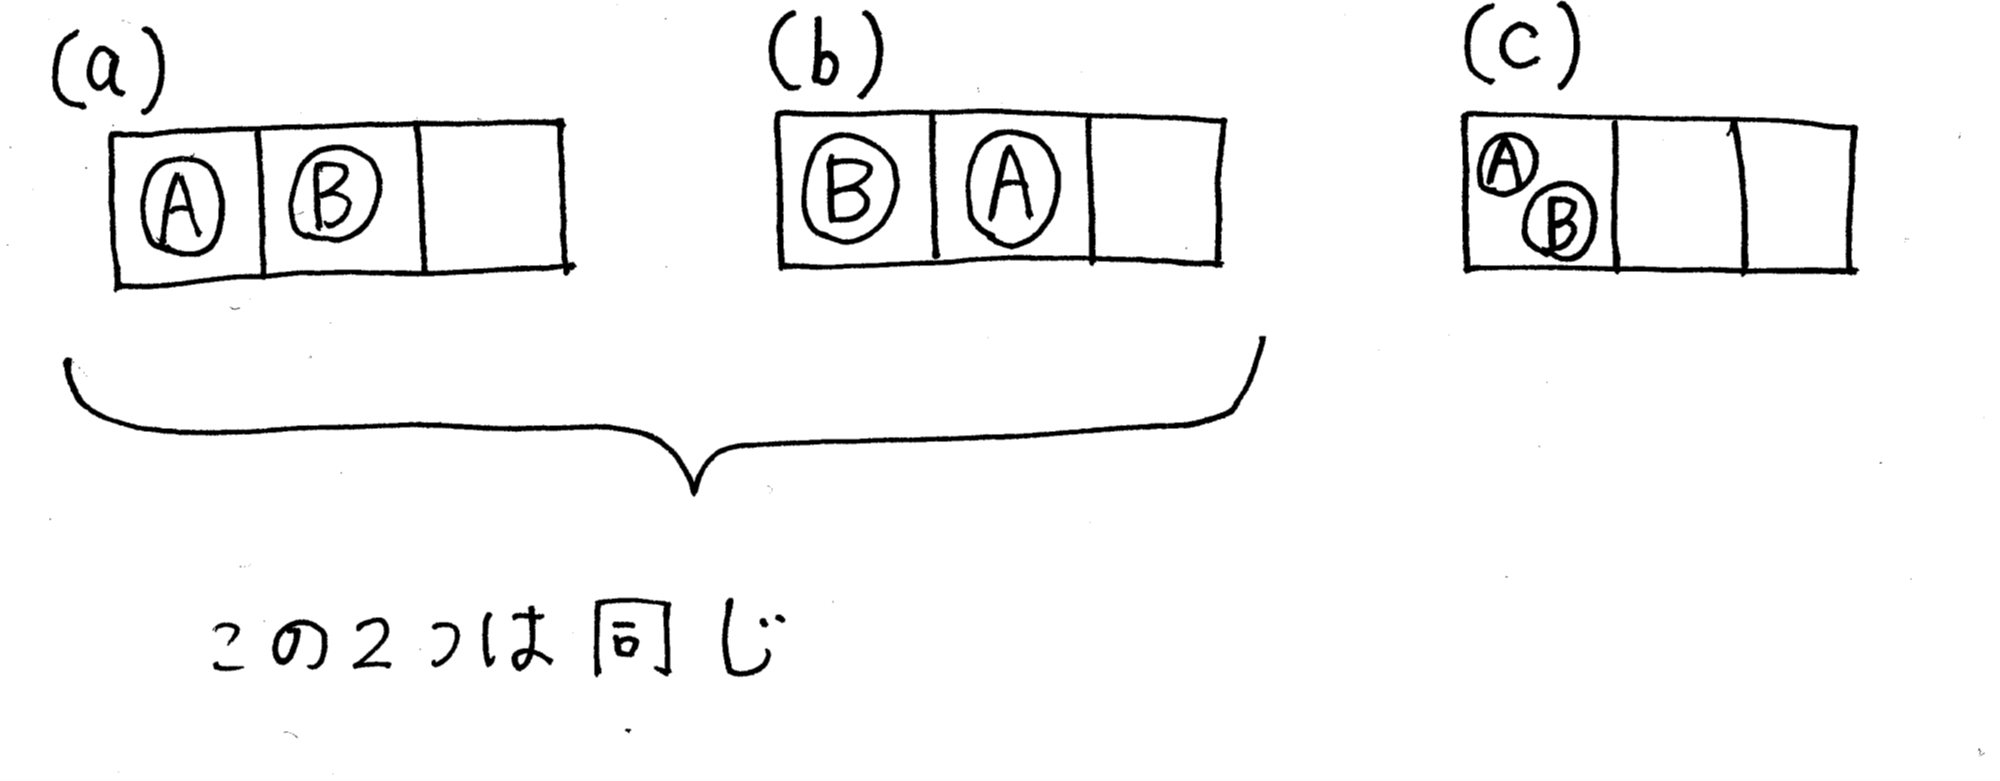
\includegraphics[width=10cm,height=4cm]{file/basic_st/fig/bo1.png}
  \caption{2この粒子AとBを3個の箱にばらまく例.(a),(b)のばらまき方は粒子の識別不可能性から同じばらまき方である.(c)は重複を許すばらまき方を表す.}
  \label{g1}
\end{figure}
%


このとき$3$個の箱に重複を許して$2$個の粒子を入れるばらまき方を考えればよい.これは,3個の箱の間にある2個の仕切りと2個の粒子の,合計4個の場所から2個の粒子(or 2個の仕切り)を選ぶやり方と等価である(図\ref{g2}).それは組み合わせを使って表せば,
\begin{align}\label{}
W_s=
\left( 
\begin{array}{cc} 
4\\[5pt] 
2\\ 
\end{array} 
\right)
=\frac{4!}{2!2!}=6\text{通り}
  \end{align}
となる.\\


 \begin{figure}[H]
 \centering
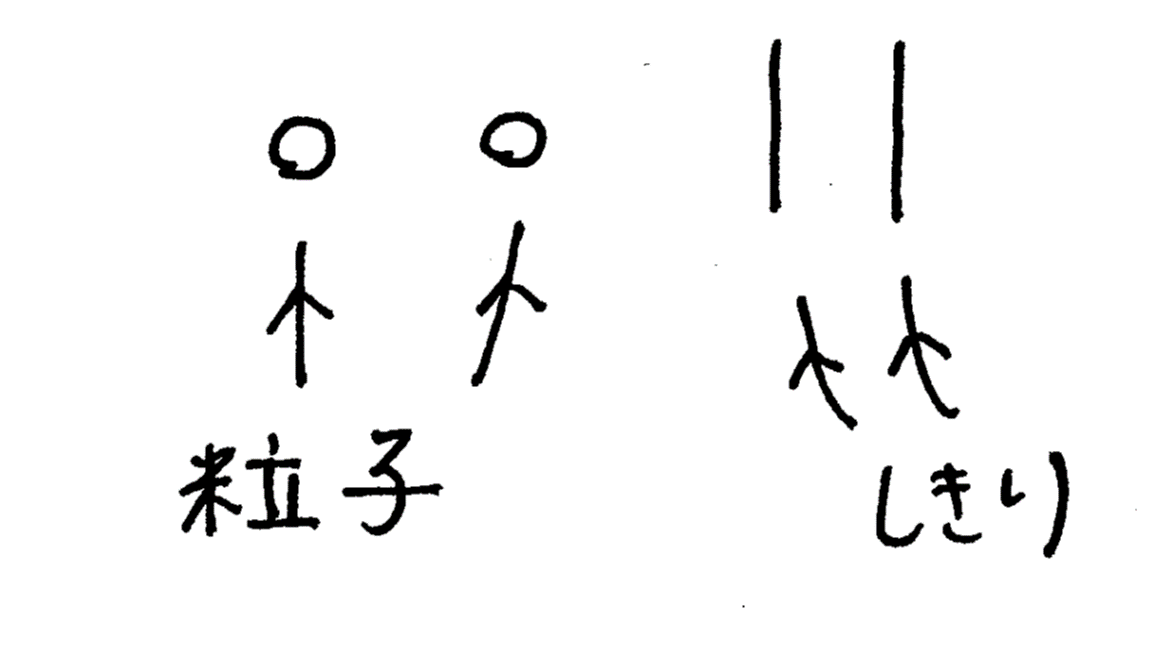
\includegraphics[width=4cm,height=2cm]{file/basic_st/fig/bo2.png}
  \caption{2個の粒子と箱の仕切り}
  \label{g2}
\end{figure}






これを一般化して表そう.$M_s$個の箱に重複を許して$N_s$個の粒子を入れる方法は,$M_s$個の箱の間にある$M_s-1$個の仕切りと$N_s$個の粒子の,合計$N_s+M_s-1$個の場所から$N_s$個の粒子(or $M_s-1$個の仕切り)を選ぶやり方と等価である.これを式で表せば,
\begin{align}\label{b1}
W_s=
\left( 
\begin{array}{cc} 
N_s+M_s+1\\[5pt] 
N_s\\ 
\end{array} 
\right)
=
\left( 
\begin{array}{cc} 
N_s+M_s+1\\[5pt] 
M_s-1\\ 
\end{array} 
\right)
=\frac{(N_s+M_s-1)!}{N_s!(M_s-1)!}
  \end{align}
となる.
\begin{figure}[H]
 \centering
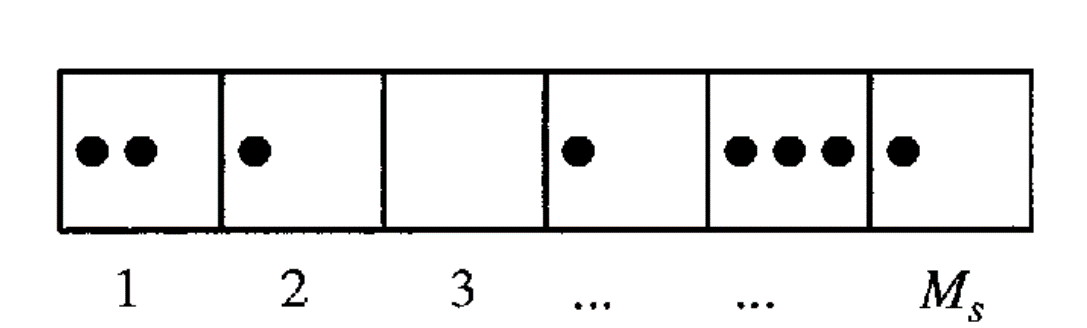
\includegraphics[width=5cm,height=2cm]{file/basic_st/fig/bo5.png}
  \caption{$M_s$個の箱に重複を許して$N_s$個の粒子を入れる方法}
  \label{g3}
\end{figure}

















%
\subsection{自由ボソンの状態密度}
簡単のため,一辺$L$の体積$V=L^3$の立方体箱に入っているスピンゼロのBose粒子を仮定する.量子力学によれば,3次元箱の中の自由粒子のエネルギー固有値,固有関数(平面波)はそれぞれ,
\be\label{d1}
\epsilon_{\bm{k}}=\frac{p^2}{2m}
=\frac{\hbar^2k^2}{2m}=\frac{(2\pi)^2\hbar^2}{2mL^2}(n_x^2+n_y^2+n_z^2)\ \ \ \ \ \ (n_x,n_y,n_z\in\mathbb{Z})\\[10pt]
\ee
\be\label{d2}
\psi_{\bm{k}}(\bm{r})\equiv\braket{\bm{r}|\bm{k}}
=\frac{1}{\sqrt{V}}\exp{(i\bm{k}\cdot\bm{r})}
=\frac{1}{\sqrt{V}}\exp{[i(k_xx+k_yy+k_zz)]}
\ee
で与えられる.3次元の周期的境界条件のもとでは,1粒子量子の波数ベクトル$\bm{k}=(k_x,k_y,k_z)$は,
\be\label{3dk}
\fbox{
$k_{x}=\left(
\dfrac{2\pi}{L}
\right)n_x,\ \ 
k_{y}=\left(
\dfrac{2\pi}{L}
\right)n_y,\ \ 
k_{z}=\left(
\dfrac{2\pi}{L}
\right)n_z$
}
\ee
で指定される.量子数$(n_x,n_y,n_z)$は整数の組である.\\
%
 $k_x,k_y,k_z$を$x,y,z$座標とする$\bm{k}$空間(波数空間)を考える.周期境界条件の下(\ref{3dk})で与えられる波数ベクトルをこの空間内で表せば,図\ref{g4}のような格子定数$2\pi/L$の単純立方格子が得られる.この単位セル一つの頂点は格子点を表す.単位セルと格子点は1対1の対応をもつ.これに注意して,$\bm{k}$空間中の微小体積$\Delta\bm{k}$中に含まれる点の数は,$\Delta\bm{k}$を単位セルの体積$(2\pi)^3/V$でわったものに等しい:
\be\label{point}
\frac{V}{(2\pi)^2}\Delta\bm{k}
\ee
ここで$\Delta\bm{k}$は単位セルに比べて十分大きいとする.これは$\Delta\bm{k}$中に存在する1粒子の取りうる状態数$M_s$を表している.



%%%%
\begin{figure}[H]
 \centering
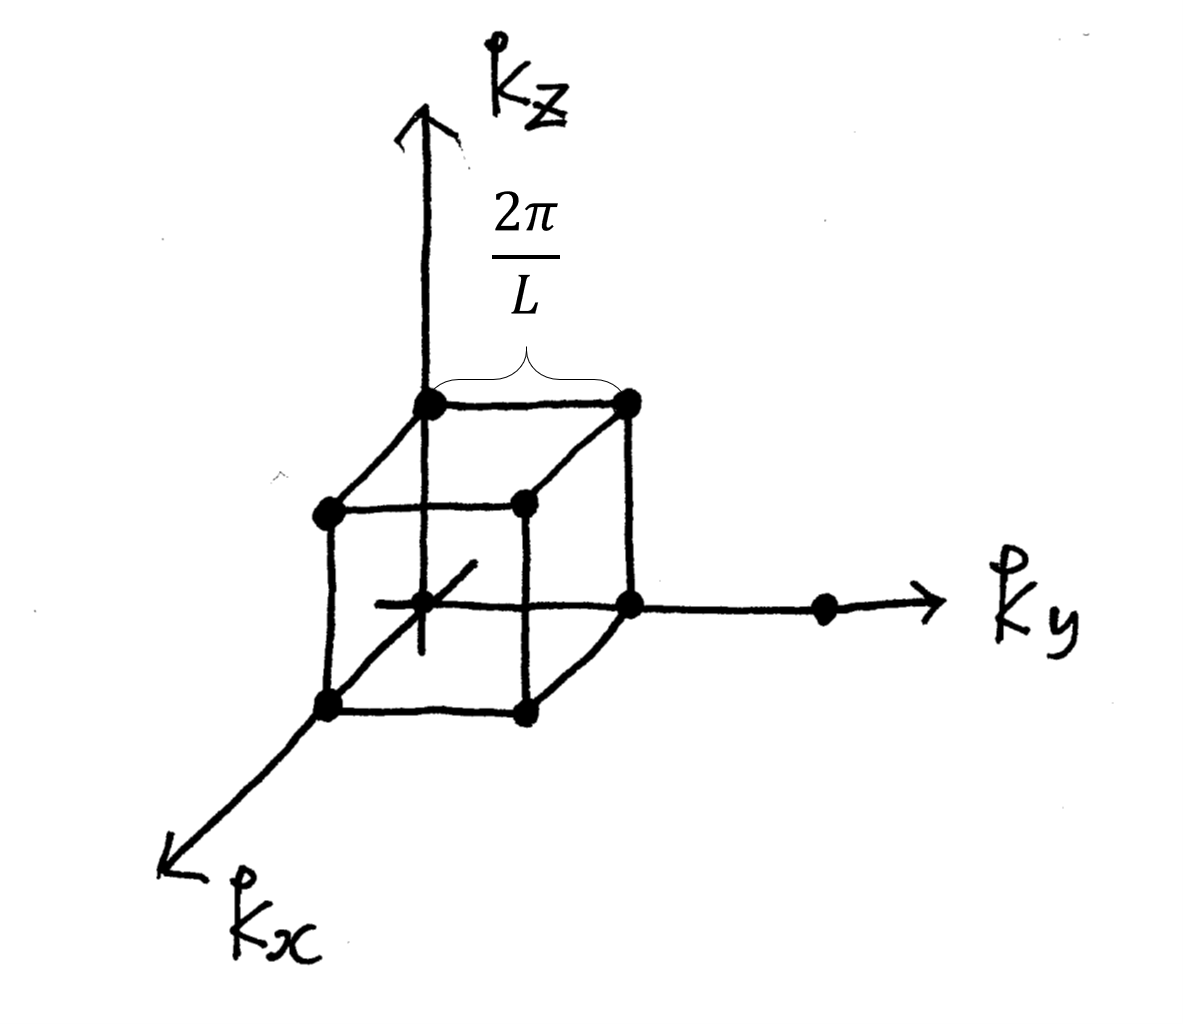
\includegraphics[width=10cm,height=8cm]{file/basic_st/fig/bo3.png}
  \caption{格子定数$2\pi/L$の単位立方格子.黒丸は格子点を表す.8個の格子点に対して,8個の単位立方格子が対応する.}
  \label{g4}
\end{figure}






$\Delta\bm{k}$を具体的に求めるには,図\ref{g5}の$[k_s,k_s+\delta k_s]$の球殻内の微小体積を考えればよい.つまり,$[k_s,k_s+\delta k_s]$の範囲にあるときの1粒子の取りうる状態数$M_s$は,殻の体積$4\pi k_s^2\delta k_s$を単位セル$(2\pi)^3/V$で割ったものに等しい:
\be\label{d3}
M_s=4\pi k_s^2\delta k_s\frac{V}{(2\pi)^3}
\ee


\begin{figure}[H]
 \centering
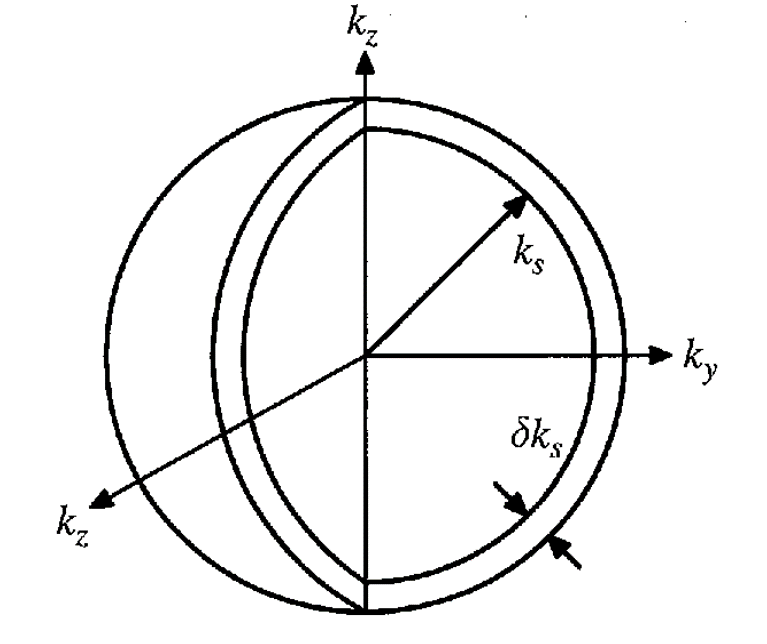
\includegraphics[width=10cm,height=8cm]{file/basic_st/fig/bo4.png}
  \caption{波数空間における領域$[k_s,k_s+\delta k_s]$の球殻}
  \label{g5}
\end{figure}





これを1粒子のエネルギーが$[\epsilon_s,\epsilon+\delta\epsilon_s]$の範囲にあるときの1粒子の取りうる状態数へ書き直す.(\ref{d1})より,波数$k_s$は
\be
k_s(\epsilon_s)=\frac{\sqrt{2m\epsilon_s}}{\hbar}
\ee
である.$\epsilon_s\to\epsilon_s+\delta\epsilon_s$と変化させたときの,波数$k_s$の微小変化$\delta k_s$は
\begin{align}
\delta k_s&\equiv k_s(\epsilon_s+\delta\epsilon_s)-k_s(\epsilon_s)
\simeq\frac{\partial k_s(\epsilon_s)}{\partial\epsilon_s}\delta\epsilon_s\nn[10pt]
&=\frac{\partial}{\partial\epsilon_s}\left(\frac{\sqrt{2m\epsilon_s}}{\hbar}\right)\delta\epsilon_s
=\frac{\sqrt{2m}}{2\hbar{\epsilon_s}^{1/2}}\delta\epsilon_s
\end{align}\label{d4}
よって,エネルギーを引数として表した波数$k_s$と$\delta k_s$を(\ref{d3})へ代入すればエネルギー空間における状態数を得る:
\begin{align}
M_s&=4\pi k_s^2\delta k_s\frac{V}{(2\pi)^3}
=4\pi\cdot\frac{2m\epsilon_s}{\hbar^2}\cdot\frac{\sqrt{2m}}{2\hbar{\epsilon_s}^{1/2}}\delta\epsilon_s\cdot\frac{V}{(2\pi)^3}\nn[10pt]
%
&=V\frac{8\pi}{(2\pi)^3}\cdot\frac{m^{3/2}{\epsilon_s}^{1/2}}{\sqrt{2}\hbar^3}\delta\epsilon_s
=\frac{Vm^{3/2}{\epsilon_s}^{1/2}}{\sqrt{2}\pi\hbar^3}\delta\epsilon_s
=Vg(\epsilon_s)\delta\epsilon_s
\end{align}
最後の等式で,$g(\epsilon_s)$を
\be
g(\epsilon_s)\equiv\frac{m^{3/2}{\epsilon_s}^{1/2}}{\sqrt{2}\pi\hbar^3}
\ee
と定義した.これを状態密度と呼ぶ.この$g(\epsilon_s)$が$\epsilon_s^{1/2}$に比例している(\ref{ep12}参照)ことは,ボーズアインシュタイン凝縮を議論するうえで極めて重要である.
%
 \begin{figure}[H]
 \centering
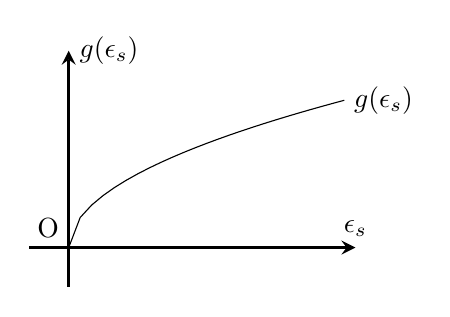
\begin{tikzpicture}
 \draw[->,>=stealth,very thick] (-0.5,0)--(pi+0.5,0)node[above]{$\epsilon_s$}; %x軸
 \draw[->,>=stealth,very thick] (0,-0.5)--(0,2.5)node[right]{$g(\epsilon_s)$}; %y軸
 \draw (0,0)node[above left]{O}; %原点
\draw[black,domain=0:3.5] plot(\x,{sqrt(\x)})node[right]{$g(\epsilon_s)$};
\end{tikzpicture}
  \label{ep12}
  \caption{$g(\epsilon_s)$は$\epsilon_s^{1/2}$に比例している.}
\end{figure}
%















%
\subsection{ミクロカノニカル集団とBoltzmannの原理}
一定の体積$V$をもち,外界と熱的・力学的相互作用のない「孤立系」を考える.この系は粒子数$N$,体積$V$,エネルギー$E$が指定される.このような熱力学系の集合はミクロカノニカル集団と呼ばれている.この熱力学系に対する熱力学ポテンシャル(状態量)はエントロピー$S$である.孤立系のエントロピー$S$は常に増加するか,または一定である.\\
 統計力学と熱力学を結び付けるために,新たな関係式を原理的に導入する.これはBoltzmannによってはじめて提唱されたもので,Boltzmannの原理と呼ばれている.
%
%
\begin{itembox}[l]{Boltzmannの原理}
実現可能な微視的状態数$W$とエントロピー$S$は次の関係式によって,与えられる.
\be\label{boltz}
S=k_{{\rm B}}\ln{W}
\ee
ここで$k_{\rm{B}}$はボルツマン定数と呼ばれている.
\end{itembox}
この関係式はマクロの量$S$とミクロな量$W$をつないでいる.\\
 孤立系のエントロピー$S$は非減少的な量であるから,系のエントロピーは可能な限り増大する.したがって,エントロピー$S$,つまり,式(\ref{boltz})が最大となるとき,熱平衡状態となる.このこと「エントロピー最大原理」として定式化しよう.
 %
%
\begin{itembox}[l]{エントロピー最大原理}
孤立系の平衡状態で非拘束変数$W$のとる値は,$W$が取りうる値の中で,全エントロピーを最大化するものに等しい.
\end{itembox}





%
\subsection{エントロピーと最大化の方法}
(\ref{boltz})を用いて,エントロピーを書き直していく.$s$番目の一つのセルについて(\ref{b1})だけのばらまき方があった.これらは独立事象であるから,全体のばらまき方は,これらの積をつくり
\be\label{s1}
W=\prod_{s}W_s
=\prod_{s}
\frac{(N_s+M_s-1)!}{N_s!(M_s-1)!}
\ee
と表される.(\ref{boltz})へ(\ref{s1})を代入する.そして,Stirlingの近似式$\ln{N!}\sim N\ln N-N$を使い,$N_s,M_s\gg1$であることを考慮すると,エントロピー$S$は
\begin{align}\label{s2}
\frac{S}{k_{{\rm{B}}}}&=\ln{W}=\ln
\left[\prod_{s}
\frac{(N_s+M_s-1)!}{N_s!(M_s-1)!}
\right]
\sim\ln
\left[\prod_{s}
\frac{(N_s+M_s)!}{N_s!(M_s)!}
\right]
\nn[10pt]
%
&\sim\displaystyle\sum_{s}[(N_s+M_s)\ln(N_s+M_s)
-(N_s+M_s)-N_s\ln{N_s}+N_s-M_s\ln{M_s}+M_s
]\nn[10pt]
%
&=\displaystyle\sum_{s}[(N_s+M_s)\ln(N_s+M_s)
-N_s\ln{N_s}-M_s\ln{M_s}
]
\end{align}
となる.\\
 孤立系で全粒子数$N$とエネルギー$E$については拘束条件
\be\label{N}
N=\displaystyle\sum_sN_s
\ee
\be\label{E}
E=\displaystyle\sum_s\epsilon_sN_s
\ee
を満たさなければならない.\\
 エントロピーの表式(\ref{boltz})における微視的状態数$W$は任意であり,このままでは使えない.だから,「何らかの方法」で平衡状態の状態数$W_{\rm{eq}}$を決める必要がある.エントロピー最大原理に従うと,この系の熱平衡状態は拘束条件(\ref{N}),(\ref{E})の条件下で,(\ref{s2})を最大化することにより得られる.このような最大化問題は「ラグランジュの未定乗数法」によって求めることができる.つまり,$\alpha$,$\beta$を「ラグランジュの未定乗数」として,関数
\be\label{s3}
f\equiv\frac{S}{k_{{\rm{B}}}}+\alpha\left(N-\displaystyle\sum_sN_s\right)+\beta\left(E-\displaystyle\sum_s\epsilon_sN_s\right)
\ee
の最大化を考えればよい.この$f$が拘束条件の条件下で最大値をとるための必要条件は
\be
\frac{\partial f}{\partial N_s}
=
\frac{1}{k_{{\rm{B}}}}\frac{\partial S}{\partial N_s}
-\alpha
-\beta\epsilon_s
=0
\ee
である.(\ref{s2})の$N_s$についての偏微分を計算し,
\begin{align}\label{s4}
\frac{1}{k_{{\rm{B}}}}\frac{\partial S}{\partial N_s}
&=\frac{\partial }{\partial N_s}
\displaystyle\sum_{s}[(N_s+M_s)\ln(N_s+M_s)
-N_s\ln{N_s}-M_s\ln{M_s}
]\\[10pt]
%
&=\ln(N_s+M_s)+1
-\ln{N_s}-1
=\ln(N_s+M_s)-\ln{N_s}=\ln\frac{N_s-M_s}{N_s}
\end{align}
まとめると,
\be
\frac{\partial f}{\partial N_s}
=
\ln\frac{N_s-M_s}{N_s}
-\alpha
-\beta\epsilon_s
=0
\ee
となる.よって,この最大化問題の解は
\be\label{s5}
\ln\frac{N_s-M_s}{N_s}=
\alpha
+\beta\epsilon_s,\ \ \ \ \ 
N_s=\frac{1}{e^{\alpha+\beta\epsilon_s}-1}M_s
\ee
と求まる.








%
\subsection{Bose-Einstein分布}
$N$粒子気体に対する熱力学第一法則
\be\label{thm}
dU=TdS-PdV+\mu dN
\ee
を使って,$\alpha,\beta$を求めよう.ここで,$T$は熱力学的絶対温度,$P$は圧力,$\mu$は化学ポテンシャルである.ここでは体積$V$が一定の場合を考えているので,
\be\label{thm1}
dU=TdS+\mu dN
\ee
となる.
これを
\be\label{thm2}
dS=\frac{1}{T}(dU-\mu dN)
\ee
と書き直す.
\be
\frac{\partial S}{\partial N_s}=k_{\rm{B}}\alpha+k_{\rm{B}}\beta\epsilon_s
\ee
\begin{align}
dS&=\displaystyle\sum_s\frac{\partial S}{\partial N_s}dN_s
=k_{\rm{B}}\displaystyle\sum_s(\alpha+\beta\epsilon_s)dN_s\\[10pt]
&=k_{\rm{B}}(\beta dU+\alpha dN)=k_{\rm{B}}\beta dU+k_{\rm{B}}\alpha dN
\end{align}
となる.ここで,$dN=\displaystyle\sum_sdN_s,dU=\displaystyle\sum_s\epsilon_sdN_s$を用いた.上式と(\ref{thm2})を比較すれば,
\begin{align}
\beta&=\frac{1}{k_{\rm{B}} T}\\[5pt]
\alpha&=-\beta\mu
\end{align}
解(\ref{s5})へ$\alpha$を代入し,$f_{\rm {BE}}(\epsilon_s)\equiv N_s/M_s$とおけば,Bose-Einstein分布
\be
\fbox{$
f_{\rm {BE}}(\epsilon_s)=\dfrac{1}{e^{\beta(\epsilon_s-\mu)}-1}
$}
\ee
を得る.この分布の意味を述べよう.この分布は1粒子状態$s$を占有する平均粒子数という物理的意味をもつ.














%
\section{グランドカノニカル集団}
\subsection{グランドカノニカル分布と大分配関数}
一つの孤立系を着目系と大きな外部系の二つに分ける.つまり,図\ref{g5}のように,(エネルギー$E$,粒子数$N$で指定される)着目系が,熱・粒子浴という大きな外部系とエネルギーと粒子の交換を許されている場合を考える.このように,外部との間に,熱に加えて粒子のやり取りがある系を「開放系」という.これで巨視的な状態として化学ポテンシャル$\mu$,体積$V$,温度$T$を指定したことになる.この系に対する集団はグランドカノニカル集団と呼ばれる.\\
%
 \begin{figure}[H]
 \centering
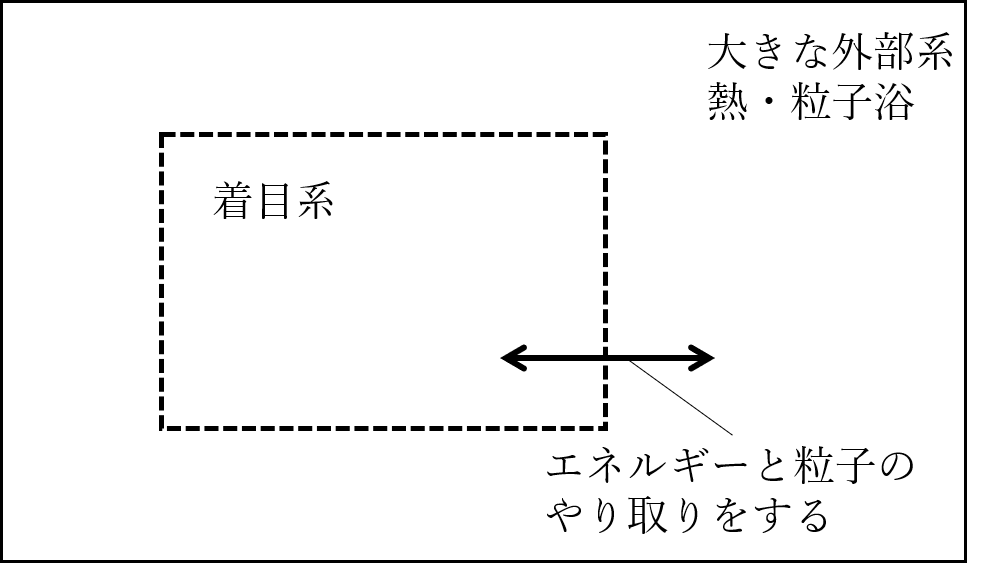
\includegraphics[width=6cm,height=4cm]{file/basic_st/fig/bo6.png}
  \caption{大きな外部系とエネルギーと粒子のやり取りをする着目系}
  \label{g6}
\end{figure}




上の設定において,着目系の粒子数$N$を一つ選ぶ,またそれに対応するエネルギー固有状態$i=1,2,\ldots,n_N$を一つ固定する.着目系がある粒子数が$N$のとき,エネルギー固有状態$i$をとる確率は,
\be
P^{(N)}_i=\frac{1}{{\it{\Xi}}}\exp\Bigl[
-\beta(E_i^{(N)}-\mu N)
\Bigr]
\ee
ここで,$E_i^{(N)}$は粒子数が$N$のときの,エネルギー固有値である.また,${\it{\Xi}}$は大分配関数と呼ばれており,次式で与えられる:
\be
{\it{\Xi}}=
\displaystyle\sum_N
\displaystyle\sum_i
\exp\Bigl[
-\beta(E_i^{(N)}-\mu N)
\Bigr]
\ee
上の二式から分かる通り,確率$P^{(N)}_i$は温度$T$と化学ポテンシャル$\mu$をパラメータとして含んでいる.



%
\subsection{グランドカノニカル集団の熱力学ポテンシャル}
グランドカノニカル集団に属する系の熱力学ポテンシャルはグランドポテンシャルと呼ばれており,次式で表される:
\be
{\it\Omega}(T,V,\mu)=-k_{\rm{B}} T\ln{{\it{\Xi}}}
\ee
これは大分配関数${\it{\Xi}}$と熱力学量であるグランドポテンシャル${\it\Omega}$を結ぶ公式である.\\
 グランドポテンシャル${\it\Omega}$の微小変化が
\be
d{\it\Omega}=-SdT-PdV-Nd\mu
\ee
と表されることを用いれば,エントロピー$S$,圧力$P$,粒子数$N$は次の熱力学関係式から得ることができる:
\be
\left(
\frac{\partial{\it\Omega}}{\partial T}
\right)_{V,\mu}
=-S,\ \ \ 
\left(
\frac{\partial{\it\Omega}}{\partial V}
\right)_{T,\mu}
=-P,\ \ \ 
\left(
\frac{\partial{\it\Omega}}{\partial \mu}
\right)_{T,V}
=-N
\ee


\subsection{バルク極限(熱力学的極)に関する注意点}
グランドポテンシャルの関係式
\be
{\it\Omega}(T,V,\mu)=-k_{\rm{B}} T\ln{{\it{\Xi}}}
\ee
は系の熱的な変化に対して,グランドポテンシャル${\it\Omega}$と大分配関数の対数$\ln{{\it{\Xi}}}$の同等性を表しているに過ぎない.他の粒子数や体積に関する変化に対しては,バルク極限(熱力学的極限)が保たれている範囲でのみこの関係式の正当性が成り立つ.バルク極限とは次の条件である:
\be
N\to\infty,\ \ \ \ 
V\to\infty,\ \ \ \ 
\frac{N}{V}=n\text{(粒子数密度)}=\text{一定}
\ee
すなわち,本来は単位体積当たりのグランドポテンシャル
\be
\frac{{\it\Omega}(T,V,\mu)}{V}=\omega(T,V,\mu)
\ee
として,次のように定式化する必要がある:
\be
\omega(T,V,\mu)
\equiv
-\lim_{V\to\infty}\frac{k_{\rm{B}} T}{V}\ln{{\it{\Xi}}},\ \ \ \ 
\text{ただし}
N\to\infty,\ \ \ \ 
\frac{N}{V}=n\text{(粒子数密度)}=\text{一定}
\ee






\bibliographystyle{unsrt}%参考文bibliographystyle献出力スタイル
\bibliography{myrefs}
\end{document}





